\documentclass[10pt]{article}

\usepackage{fullpage}
\usepackage{color}
\usepackage[table]{xcolor}
\usepackage{hyperref}
\usepackage{graphicx}

%%%%%%%%%%%%%%%%
% Miscellaneous
%%%%%%%%%%%%%%%%

\definecolor{primary}{rgb}{0,0,.50}
%\definecolor{primary}{rgb}{0,0,0}
\definecolor{secondary}{rgb}{.7,.5,0}
\definecolor{table-primary}{rgb}{1,1,1}
\definecolor{table-secondary}{rgb}{.975,.99,1}

%%%%%%%%%%%%%%%%
% Title Section
%%%%%%%%%%%%%%%%

\title{\color{primary}\texttt{UCSC Plaza \\ Sprint3 Review Report}}
\author{{\color{secondary}\textbf{Team Amlesh the Great}} \\ Kyungmin So (PO), Youngsoo Jang, \\ Hobin Ryu, Seungwoo Lee \\ Amlesh Sivanantham, and James Garbagnati }

%%%%%%%%%%%%%%%%%%%%%%
% User-Defined Macros
%%%%%%%%%%%%%%%%%%%%%%

%\ignore = Multiline comments
\newcommand{\ignore}[1]{}

\newcommand{\gobblepagenum}{\thispagestyle{empty}\addtocounter{page}{-1}}

%\fancysec{Section title}{Label} = Fancy, colored and labelled section
% Basically just to make it easier to change the format of the whole doc
% Commands with an X are non-numbered sections
\newcommand{\fancysec}[2] {{\color{primary}\section{#1} \label{sec:#2}}}
\newcommand{\fancysub}[2] {{\color{primary}\subsection{#1} \label{sec:#2}}}
\newcommand{\fancysubsub}[2] {{\color{primary}\subsubsection{#1} \label{sec:#2}}}

\newcommand{\fancysecX}[2] {{\color{primary}\section*{#1} \label{sec:#2}}}
\newcommand{\fancysubX}[2] {{\color{primary}\subsection*{#1} \label{sec:#2}}}
\newcommand{\fancysubsubX}[2] {{\color{primary}\subsubsection*{#1} \label{sec:#2}}}


% P.S. I'm so fancy, you already know


%%%%%%%%%%%%%%%%%
% Begin Document
%%%%%%%%%%%%%%%%%
\begin{document}

\maketitle
    
\fancysecX{Actions to stop doing}{stop}
     
        \begin{itemize}
            \item None.
        \end{itemize}    

\fancysecX{Actions to start doing}{start}
        \begin{enumerate}
            \item Our team should ensure our whole product is polished.
            \item Our team should begin more unit testing and create automated unit testing.
            \item Our team should practice better git practices so as to avoid merge conflicts (of which we have not had many).
        \end{enumerate}  

\fancysecX{Actions to keep doing}{keep}
     
    \begin{enumerate}
        \item Finishing up the leftover work from sprint 2...
	\end{enumerate}

\fancysecX{Work completed/not completed}{completeWork}

	\fancysubX{Work completed}{completed}
		\begin{itemize}
            \item User Story 1
            \item User Story 2
            \item User Story 3
            \item User Story 5
            \item User Story 7
            \item User Story 8
            \item User Story 9
    	\end{itemize}

    \fancysubX{Work not completed}{notCompleted}
		\begin{itemize}
            \item User Story 6
    	\end{itemize}

\fancysecX{Work completion rate}{completeRate}

	\begin{itemize}
            \item Total number of user stories completed during sprint 2: 7 User stories
    \end{itemize}

    \begin{itemize}
            \item Total number of estimated ideal work hours completed during sprint 2: 23 hours
    \end{itemize}

    \begin{itemize}
            \item Total number of days during sprint 2: 7 days
    \end{itemize}


    \begin{figure}[!ht]
  	
  	\centering
    		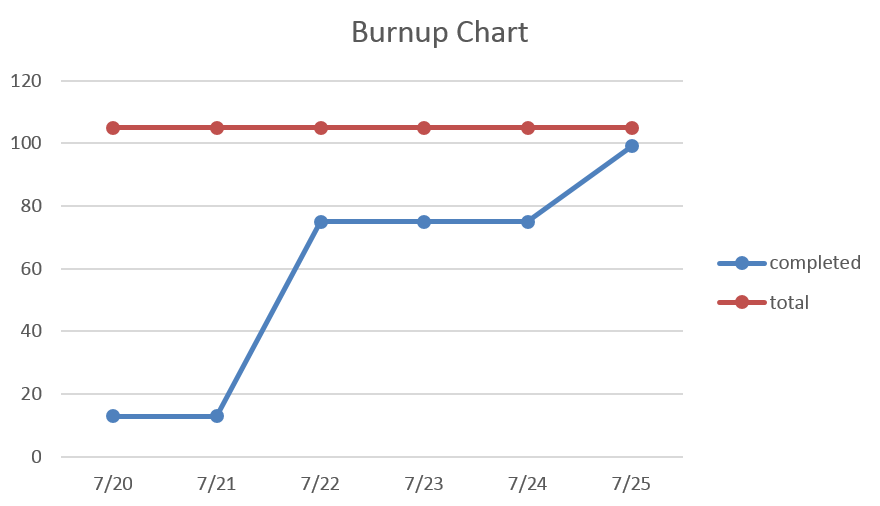
\includegraphics[width=1\textwidth]{Burnupchart3}
    \caption{Burnup Chart at the end of sprint 3}
    \end{figure}

\vspace{5cm}


\end{document}
